\documentclass[a4paper,12pt]{article}
\usepackage[a4paper, margin=2.54cm]{geometry}
\usepackage[german]{babel}
\usepackage[UTF8]{inputenc}
\usepackage{setspace}
\usepackage{graphicx}
\usepackage{caption}
\usepackage{subcaption}
\onehalfspacing

\usepackage{listings}

\lstdefinelanguage
[x64]{Assembler}     % add a "x64" dialect of Assembler
[x86masm]{Assembler} % based on the "x86masm" dialect
% with these extra keywords:
{morekeywords={CJNE,CDQE,CQO,CMPSQ,CMPXCHG16B,JRCXZ,LODSQ,MOVSXD, %
		POPFQ,PUSHFQ,SCASQ,STOSQ,IRETQ,RDTSCP,SWAPGS, %
		rax,rdx,rcx,rbx,rsi,rdi,rsp,rbp, %
		r8,r8d,r8w,r8b,r9,r9d,r9w,r9b, %
		r10,r10d,r10w,r10b,r11,r11d,r11w,r11b, %
		r12,r12d,r12w,r12b,r13,r13d,r13w,r13b, %
		r14,r14d,r14w,r14b,r15,r15d,r15w,r15b}} % etc.
\usepackage{xcolor}
\lstset {
	language=[x64]Assembler,
	keywordstyle=\color{blue},
	numbers=left, 
	numberstyle=\small, 
	numbersep=8pt, 
	frame = single, 
}

\begin{document}

	\section{Einführung}
	\subsection{Motivation}
	In der heutigen Zeit wird der Verwendung von Mikrocontrollern eine immer höre Bedeutung zugemessen. Diese entsteht durch die einfache Programmierung auf Systemebene in Assebly sowie die konstengünstige und platzspaarende Produktion.\\
	Die Verwendung des 8051  bietet hierbei eine bekannte Plattform, welche sich für die Umsetzung einer Vielzahl an kreativen Projekten eignet.\\
	Die Idee dieses Projektes besteht darin, die Hardware mit verschiedener Peripherie zur Eingabe von Morse-Code zu nutzen.\\
	Der Morse Code ist ein Code, welcher zur Übermittlung von Daten in Textform genutzt werden kann und die Verständigung über primitive Technik erlaubt. 
	\subsection{Aufgabenstellung}
	Die Aufgabenstellung war es ein Programm für den 8051 Microcontroller zu schreiben, das folgende Anforderung erfüllt:
	\begin{itemize}
		\item Compilierfähigkeit des Programmes
		\item Verwendung eines Timers
		\item Verwendung eines Interrupt
	\end{itemize}
	Zur Vereinfachung wurde anstatt eines 8051 ein Simulationsprogramm verwendet, welche sowohl den 8051, als auch die Ein und Ausgabehardware simuliert.\\
	Der fertige Code ist offen auf Github zu finden.
	
	\newpage
	
	\section{Grundlagen}
	\subsection{Assembler}
	Als Assembler oder Assebly bezeichnet man eine Programmiersprache, mit welcher sich eine bestimmte Hardware oder Prozessorachitektur gezielt programmieren lässt. Asseblercode wird also gezielt für eine Architektur entwickelt und lässt sich nur auf dieser ausführen.\\
	Der Quellcode bildet hierbei eine Folge von Maschinenbefehlen. Maschinenbefehle bestehen dabei aus einem Operationscode und meist einer weiteren Folge von Angaben wie Adressen oder Literalen.\\
	\ref{ls:mov} zeigt hierbei einen einfachen MOV - Befehl in  der Maschinensprache von x86 Prozessoren. MOV bedeutet hierbei so viel wie mov-byte von/was, nach. Verschiedene Assembler Dialekte unterscheiden sich in der Bedeutung gleicher Befehle.\\
	
	\subsection{8051 Mikrocontroller}
	Der Intel 8051 ist ein von in den Jahren von 1980 bis 1990 unter anderen von Intel und Simens hergestellter Mikrokontroller. Verwendung fand er in unbterschiedlichen Gebieten der Automobilindustrie, Robotik sowie der Telekommunikation.\\
	In der ursprünglichen und hier betrachteten Form handelt es sich bei dem 8051 um einen Rechner nach der Havard-Architektur \cite, welche den Programm vom Datenspeicher trennt.\\
	Der Prozessortakt ist mit 12MHz und der Befehlsatz mit 8 Bit = 1 Byte angegeben. Außerdem verfügt er über einen 4 KB Programmspeicher, 128 Byte Datenspeicher und zwei 16-Bit Timer. Andere Prozessoren der Baureihe können auch leistungsfähiger sein.\\

	
	
	\subsection{Entwicklungsumgebung MCU 8051}
	Zur Implementierung des Programms wurde nicht direkt an der Hardware des 8051 gearbeitet, sondern mit einer virtuellen Entwicklungsumgebung des 8051, der MCU 8051 von Mavriria Microsystems.\\
	Vorteile des Einsatz der Virtuellen Hardware war der direkte Einblick in die verschiedenen Register und Ports des 8051 sowie der virtuellen Hardware. 
	\begin{figure}[bt]
		\centering
		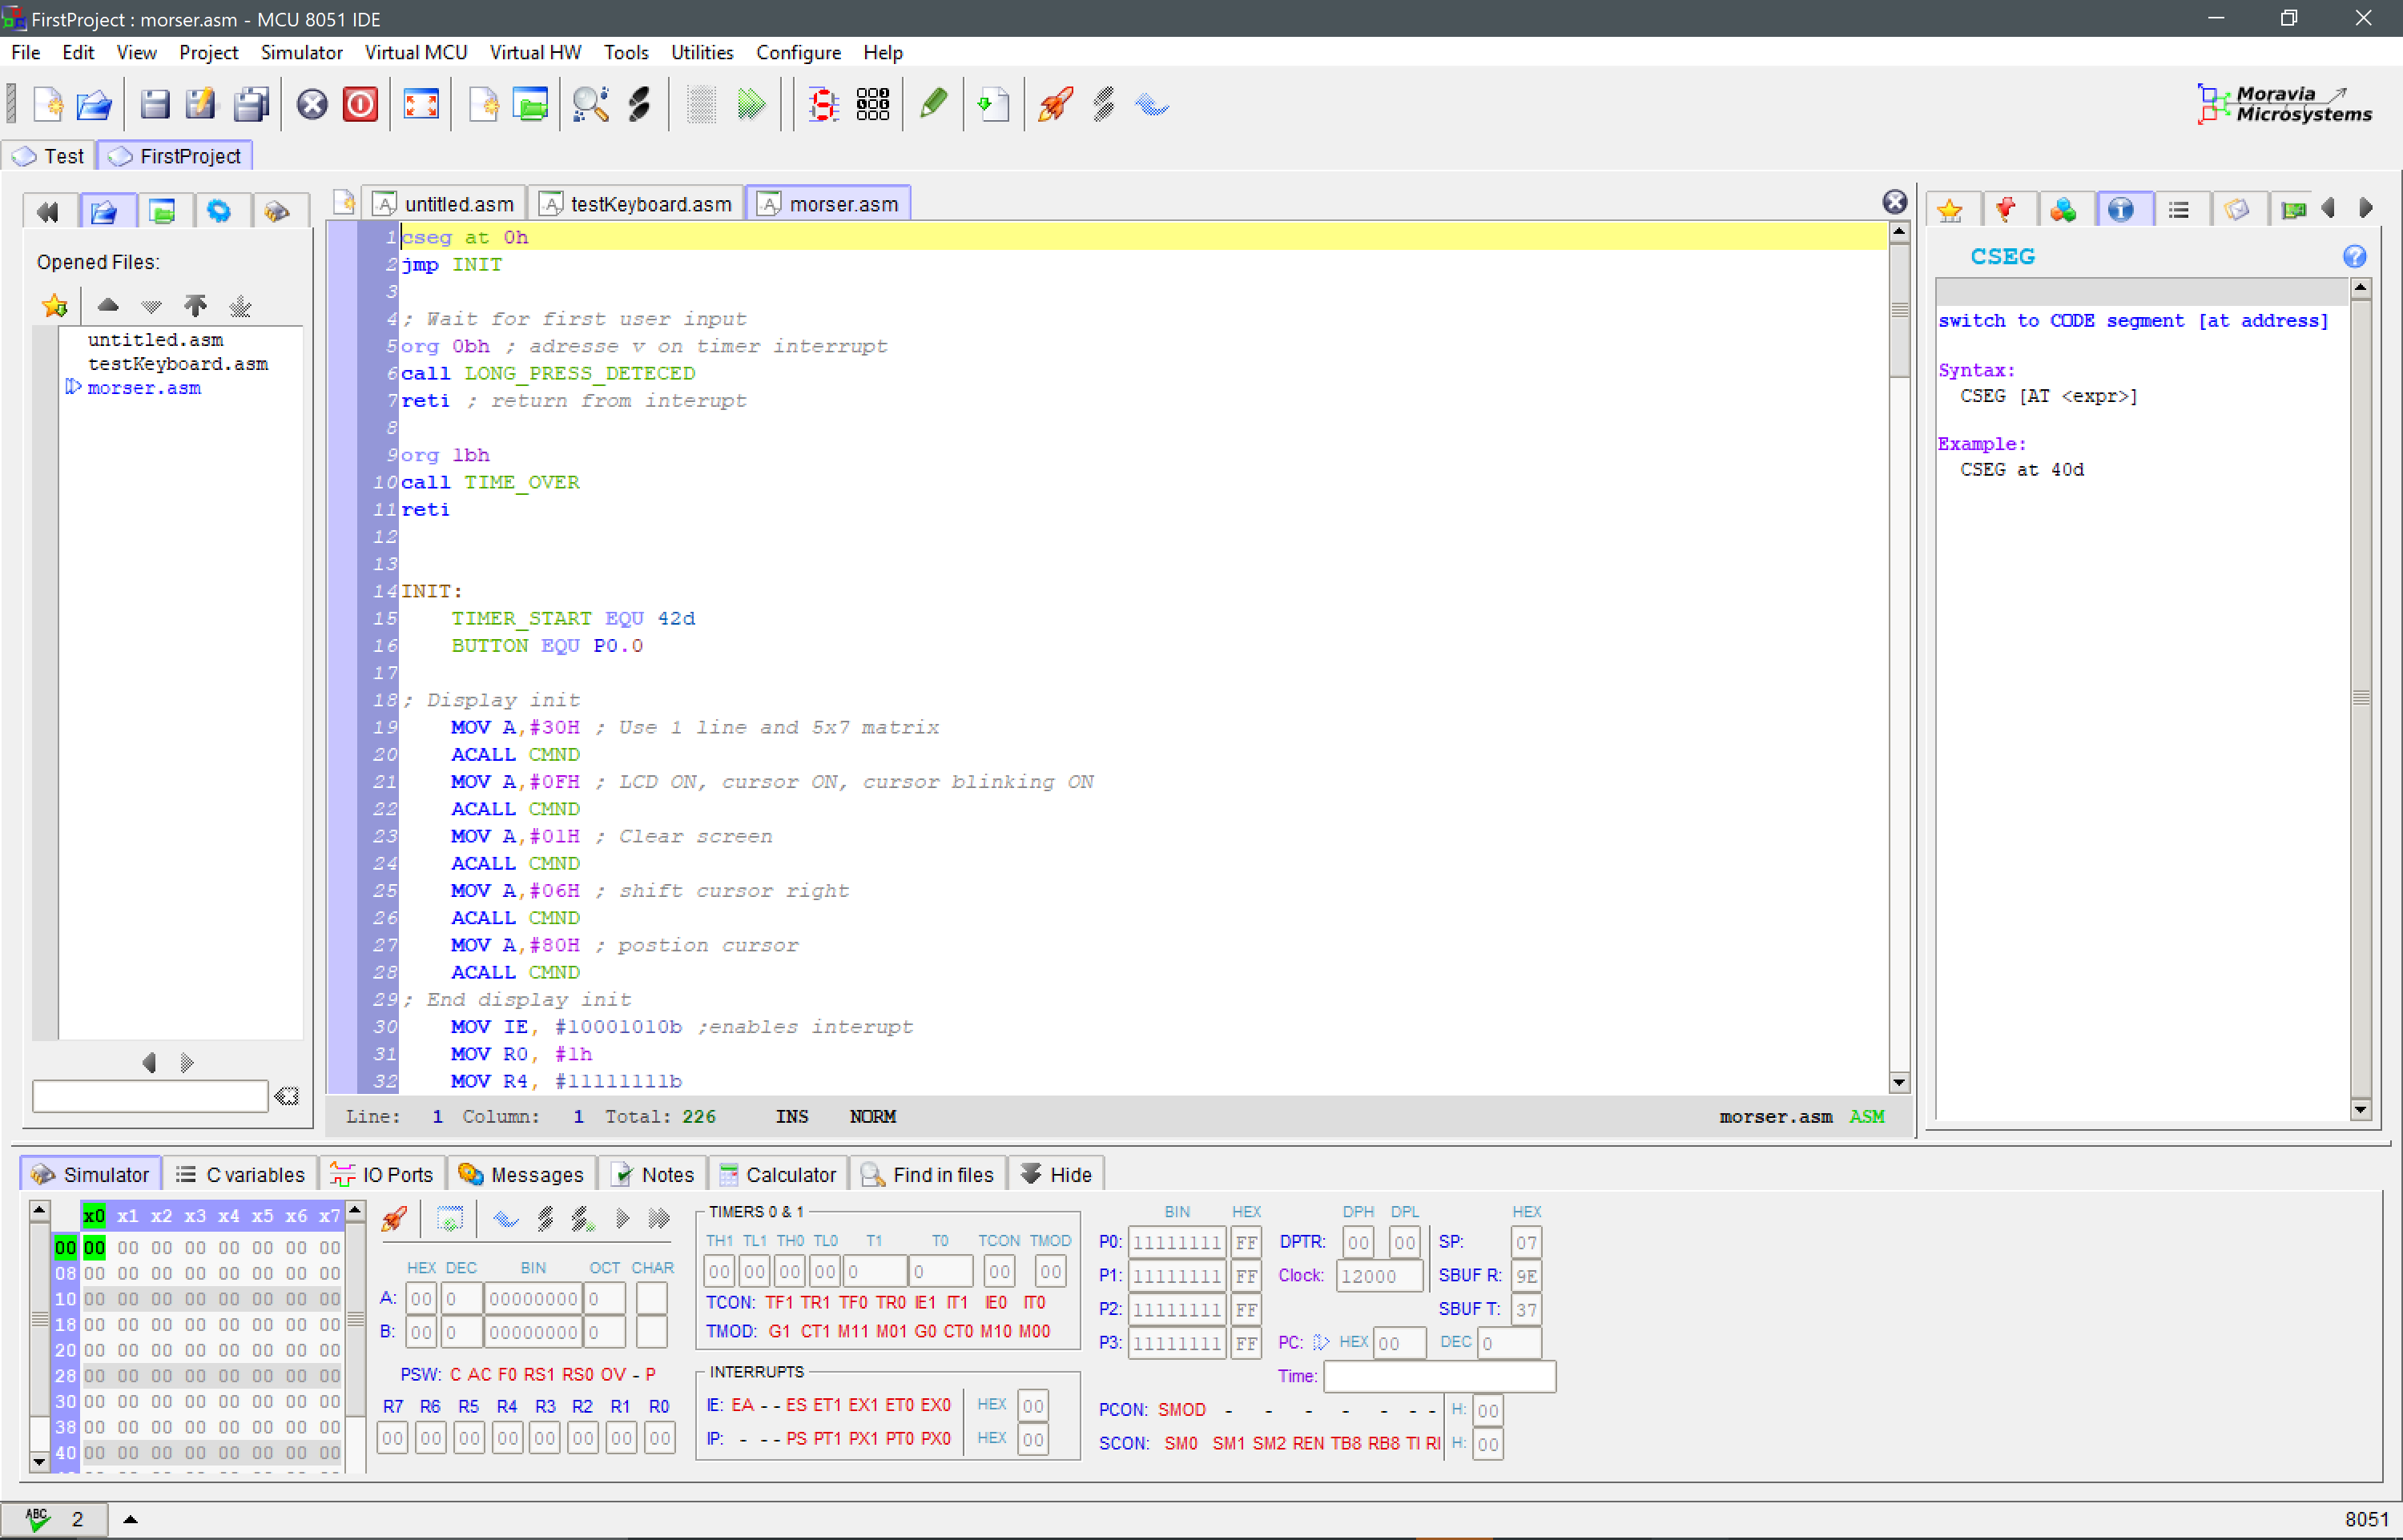
\includegraphics[width=0.7\linewidth]{Bilder/IDE8051}
		\caption[IDE Screenshot]{IDE Screenshot}
		\label{fig:ide8051}
	\end{figure}

	Im Folgenden geben wir ein Übersicht der Virtuellen Hardware, welche für das Projekt verwendet wurde.
	\subsubsection{Simple Keypad}
	\begin{figure}[bt]
		\centering
		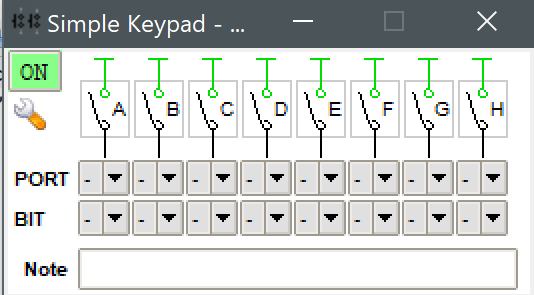
\includegraphics[width=0.7\linewidth]{Bilder/keypad}
		\caption[IDE Screenshot]{Simple Keypad in IDE}
		\label{fig:ide8051keybad}
	\end{figure}
	Mit dem Simple Keypad \ref{ide8051keybad} lassen sich über dedizierte Ports jeweils Schalter simulieren, welche entweder an oder aus sind. 
	
	\subsubsection{LC Display}
	\begin{figure}[bt]
		\centering
		\includegraphics[width=0.7\linewidth]{Bilder/lcd}
		\caption[IDE Screenshot]{LCD in der IDE}
		\label{fig:ide8051lcd}
	\end{figure}
	Das verwendete LC Display ist ein 8x1 Display mit einer HD44780 Steuereinheit. Das HD44780 verwendet 11 Ports zur Steuerung
	
	\begin{tabular}{l|c|l}
		Bit & Input/Output & Erklärung \\ \hline
		RS & I & 0 = Befehl, 1 = Daten \\
		R/W & I & 0 = schreiben, 1 = lesen \\
		E & I & Enable \\
		D0 & I/O & Daten-Bit 0 (LSB) \\
		D1 & I/O & Daten-Bit 1 \\
		D2 & I/O & Daten-Bit 2 \\
		D3 & I/O & Daten-Bit 3 \\
		D4 & I/O & Daten-Bit 4 \\
		D5 & I/O & Daten-Bit 5 \\
		D6 & I/O & Daten-Bit 6 \\
		D7 & I/O & Daten-Bit 7 (MSB)
	\end{tabular}\\
	
	Das Enable bit wird dazu verwendet um anzuzeigen, dass der derzeitig angelegte Zustand an das Display gesendet werden soll. Um einen Befehl an das zu senden müssen RS und R/W Bit jeweils 0 sein. Dabei wird der wert auf den Daten Bits als Befehl interpretiert. Um Daten auf das Display zu senden wie zum Beispiel einen Buchstaben muss RS 1 sein, R/W 0 und auf den Datenbits muss der Wert des Buchstaben als ASCII Zeichen anlegen. Eine wichtige Eigenschaft des Displays ist, dass Befehle immer eine gewisse Zeit zum ausführen brauchen. Deshalb gibt es eigens dafür ein Busy-Flag welches angibt, ob das Display noch an seinem letzten Befehl arbeitet. Dieses kann gelesen werden, indem man RS auf 0 und R/W 1 auf eins setzt. D7 enthält dann den wert das Busy-Flags.

	\subsection{Morsecode}
	Der Morsecode [\ref{fig:morse-code}] ist ein Zeichensatz, welcher zu Übertragung von Daten verwendet wird. Das Morsealphabet besteht dabei aus drei dijunkten Zeichen: kurzes Signal, langes Signal, Pause. Das bekannteste Morsesignal ist \textit{kurz - kurz - kurz - lang - lang - lang - kurz - kurz - kurz}, welches für den Seenotruf SOS steht. Das Signal kann dabei als Tonsignal, als Funksignal oder als elektischer Impuls von einem Morsetaster über eine Telefonleitung, mechanisch oder optisch übertragen werden.\\
	Der Morsecode ist eine Entropiekodierung, da öfters vorkommende Zeichen mit weniger Signalen codiert sind (ausgehend von der Häufigkeit in der englischen Sprache).\\

	\begin{figure}[bh]
		\begin{subfigure}{0.5\linewidth}
			\centering
			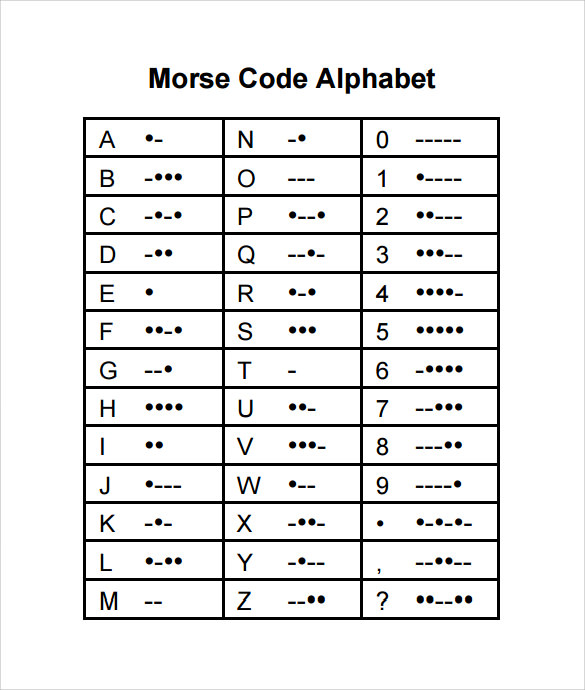
\includegraphics[width=0.95\linewidth]{Bilder/Morse-Code-Alphabet-Chart.jpg}
			\caption{Internationaler Morse Code}
			\label{fig:morse-code}
		\end{subfigure}
		\begin{subfigure}{0.5\linewidth}
			\centering
			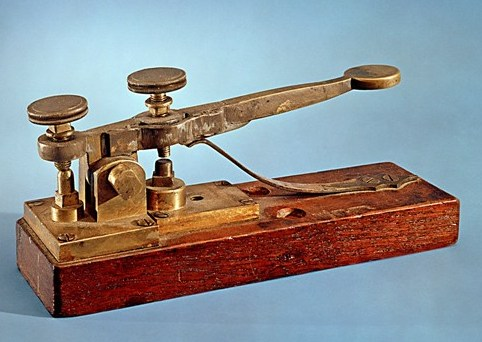
\includegraphics[width=0.95\linewidth]{Bilder/morse-telegraph-machine.jpg}
			\caption{Morsecode-Telegraph}
			\label{fig:morser}
		\end{subfigure}
	\end{figure}

	Unzulänglichkeiten des Morse-Codes bestehen darin, dass die Fano-Bedingung für den Morse-Code nur dann enfüllt ist, wenn man das dritte Symbol, die Pause als festes Symbol definiert. Daraus ergibt sich, dass keine Wort den identischen Anfang eines anderen Wortes ist. Nach jedem erkannten Wort kann also direkt mit dem nächsten Wort weitergemacht werden.
	
	\newpage 
	\section{Konzept}
	\subsection{Analyse}
	Ein wichtiger Bestandteil des Programms ist die richtige Interpretation der Eingabe. Dafür ist es wichtig, zwischen einem kurzen und langen drücken zu lernen. Zusätzlich muss erkannt werden, dass die Eingabe vorbei ist, dass also das Zeichen Pause eingegeben wurde, wenn nichts mehr gedrückt wird oder das 4te mal eine Eingabe erfolgt ist, da dies die Maximallänge einer möglichen Eingabe ist. Die Eingabe muss abgespeichert werden und dann in den zur Eingabe passenden Buchstaben decodiert werden. Dieser Buchstabe muss dann an das LC Display gesendet und dort angezeigt werden. Nach einem interpretierten Buchstaben muss der Nutzer in der Lage sein können, eine erneute Eingabe zu tätigen.\\
	\subsection{Zustände}
	Aus der obrigen Analyse ergeben sich folgende Zustände:
	\begin{enumerate}
		\item[Z1] Der Nutzer hat noch keine Eingabe getätigt und der Automat wartet auf eine Eingabe
		\item[Z2] Der Nutzer drückt den Morseknopf.
		\item[Z3] Abhängig von der Dauer, die der Nutzer den Knopf gedrückt hält, wird dieser als langes oder kurzes Signal interpretiert
		\item[Z4] Der Automat wartet wieder auf eine Eingabe. Erfolg eine Eingabe, folgt Z2. Ohne Eingabe läuft ein Timer ab.
		\item[Z5] Der Timer ist abgelaufen und die bisherige Eingabe wird interpretiert und das Ergebnis wird angezeigt.
	\end{enumerate}

	\begin{figure}
		\centering
		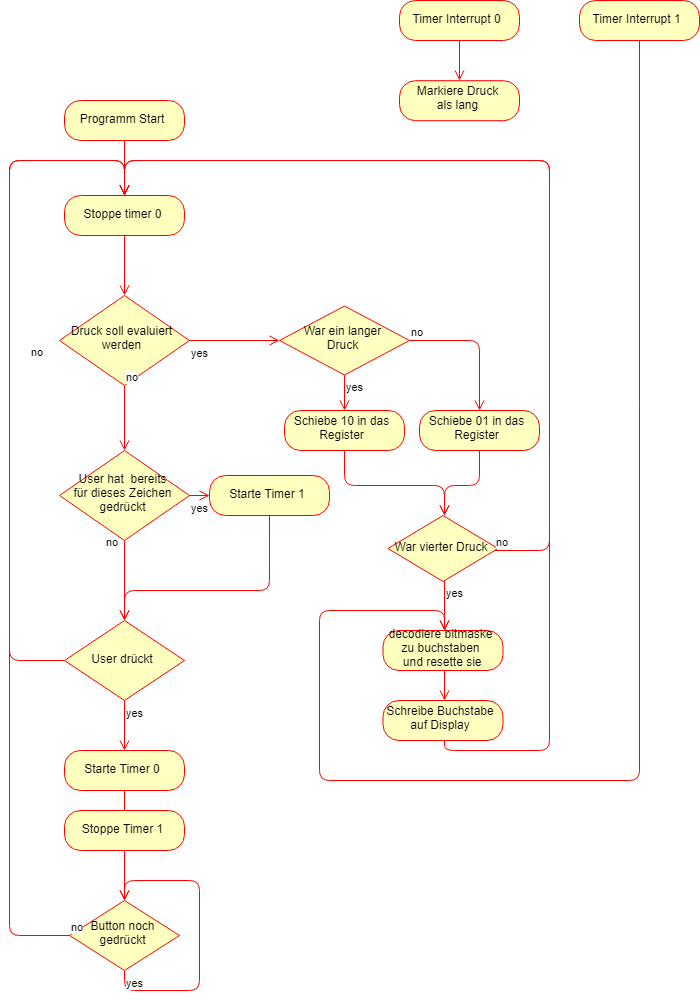
\includegraphics[width=0.8\linewidth]{Bilder/Programmablaufplan}
		\caption[Programmablauf]{Programmablauf}
		\label{fig:programmablaufplan}
	\end{figure}

	\newpage
	\section{Implementierung}
	\subsection{Initialisierung des Displays}
	 Damit das Display richtig bedienbar ist müssen einige Initialisierungsschritte vorgenommen werden. Mit dem Befehlswert \#30H sagen wir der dem Display das wir eine Zeile mit 5x7 Matrizen als Anzeige für ein Zeichen verwenden wollen. Als nächstes schalten wir das Display ein und aktivieren den Cursor und setzen ihn blinkend mit dem Code \#0FH. Um mögliche Überbleibsel von vorherigen Verwendungen auf dem Display zu entfernen senden wir zusätzlich den Code \#01H welcher das den Inhalt des Displays zurücksetzt. Anschließend wird mit den Befehlen \#06h und \#80h der Cursor auf den Anfang des Displays positioniert.

	\subsection{Schleifen}
		\begin{lstlisting}[caption={Dauerschleife während Knopf nicht gedrückt ist},captionpos=b]
	CLR tr0
	CJNE R0, #1h, ANALYZE_PREV
	;Run timer to detect break
	CJNE R5, #0h, START_WAIT_TIMER
	JNB BUTTON, START_TIMER
	JMP BTN_LOOP
		\end{lstlisting}
	Nach der Initialisierung des Displays durchläuft das Programm verschiedene Schleifen. Die erste Schleife wird immer dann durchlaufen, wenn der Button auf dem Simple Keypad, welcher auf P0.0 anliegt, gerade nicht gedrückt ist. Wird dieser gedrückt, wechselt das Programm in eine andere Schleife, in welche er so lange bleibt, wie der Button gedrückt ist. Hierbei wird Timer 0 aktiviert. Wenn das Programm eine bestimmte Zeit in der pressed-Schleife bleibt, läuft der Timer ab und ein Interrupt speichert die Information, dass der letzte Knopdruck lang war.\\
	Wenn der Knof wieder losgelassen wird, landet das Programm wieder in der initialen Loop. Hier wird der Timer 0 wieder gestoppt. Diesmal läuft jedoch Timer 1 mit. Dieser ist für die Codierung des Pause Symbols zuständig. Wenn dieser abläuft, dann beginnt das encoden der Bitmaske, welche die Informationen über die bisherige Eingabe enthält. Der Timer 1 läuft nicht ab, wenn der User eine weitere Eingabe tätigt.
	
	\subsection{Bitmaske}
	 Die Eingabe des Users wird in einer Bitmaske im Register 2 gespeichert. Diese wird in einer eigenen 8-bit Bitsmaske gespeichert. Hierbei kommt die Registerlänge von 8-bit der Tatsache zu gute, dass die maximallänge eines Morse Codes 4 Zeichen sind. Es lässt sich also, \textit{01} für kurz oder \textit{10} für lang abspeichern, wenn man durch die Bits shiftet. Der Zustand \textit{00} steht für nicht verwendetet Bits und \textit{11} für einen nicht definierten Zustand. Die folgende Bitmaske steht demnach für \textit{lang - kurz}.
	 \begin{center}
		$00001001$
	\end{center}
	Diese Mitmaske wird im letzten Schritt - dem encoding - verarbeitet.
	 
	\subsection{Encodieren}
	Nun ist es notwendig die Bitmaske in einen ASCII Wert zu dekodieren, damit dieser an das Display gesendet werden kann. Dies geschieht durch eine Vielzahl von Gleichheitsabfragen für jeden Buchstaben, die den Wert der Bitmaske in A vergleichen. Wenn der Wert übereinstimmt wird mit dem MOV Befehl der Wert des Zeichens in das Register geschrieben. A hat dabei den Wert 0 und Z 25.
	\begin{lstlisting}[caption={Beispielhafte Gleihheitsabfrage für den Buchstaben A},captionpos=b]
	CJNE A, #00000110b, ENCODE_BITMASK + 6; A
	MOV R3, #0d
	\end{lstlisting}
	Anschließend wird der Wert des Register noch um 65 erhöht um den ASCII Wert zu ermitteln. Dieser wird dann an das LC Display gesendet. Sollte kein Wert übereinstimmen wird ein Default Wert von $11111111$ genommen, was einem voll ausgefüllten Kasten entspricht.

\end{document}


